\documentclass{article}
\usepackage{FinalYearProjectReport}

% packages for references
\usepackage{cite}
\usepackage{url}


% uncomment this line to double line spacing for proof reading
% \linespread{2}

% packages and settings for graphics
\usepackage[pdftex]{graphicx}
\graphicspath{{./}}
\DeclareGraphicsExtensions{.png}
\usepackage[final]{pdfpages}


\title{Traffic Reporter - Final Report}
\name{Michael Little}
\address{Department of Electrical and Computer Engineering\\
University of Auckland, Auckland, New Zealand}


\hyphenation{and-roid}


\begin{document}

\begin{titlepage}


\vspace*{15em}


\centering

{\LARGE
Department of Electrical \& Computer Engineering \\
Final Year Research Project 2013, Final Report}

\hspace{2em}

% notes on latex tables use "&" as colum sperator
\begin{table*}[h]
\centering
\begin{tabular}{ll}
Project Title: & Traffic Information Engine for Auckland Traffic Lights \\
Project Number: & 14 \\
Supervisor Name: & Dr. Nasser Giacaman \\
Second Examiner Name: & Dr. Partha Roop \\
Your Name: & Mike Little \\
Your UID: & 2626904 \\
Partner Name: & Andrew Luey \\
Date submitted: & 15 September 2013 \\

\end{tabular}
\end{table*}
\begin{table}


\end{table}
\pagebreak

\vspace*{25em}

{\Large Declaration of Originality}

\hspace{5em}

This report is my own unaided work and was not copied from 
nor written in collaboration with any other person.

Name: Mike Little


\end{titlepage}




\maketitle

\begin{abstract}

\end{abstract}

\section{Introduction}
\subsection{Objective}
Auckland Transport has an application that they use to view and analyse traffic volume. The application was last updated in 2007 and is lacking in features and usability. My partner and I were tasked with recreating this application using modern technologies with the goal of improving the features already existing in the application, and adding new features.

\subsection{Motivation}
According to the 2006 census, travel by car accounted for 48\% of travel and 44\% of travel was by public transport. Up to 2030 60\% of New Zealand's population growth is going to occur in Auckland. In terms of numbers of trips, in 2006 there were approximately 4 million trips per day in Auckland. This number is projected to grow to 5.5 million trips per day in 2041.

There is limited ability for Auckland to expand its road network so Auckland transport should focus on making their current road infrastructure more effective. A better understanding of Auckland's traffic would lead to better city planning and traffic optimization.

\subsection{Background}

At an intersection with traffic lights, under each lane there are inductive loops that can detect when a vehicle travels over them. Every 5 minutes these detectors send their counts to that intersection's traffic controller. The traffic controller sends the volume data to Auckland's SCATS server \cite{sims1981scat}. See Figure \ref{fig:background}. 

\begin{figure}[!t]
\centerline{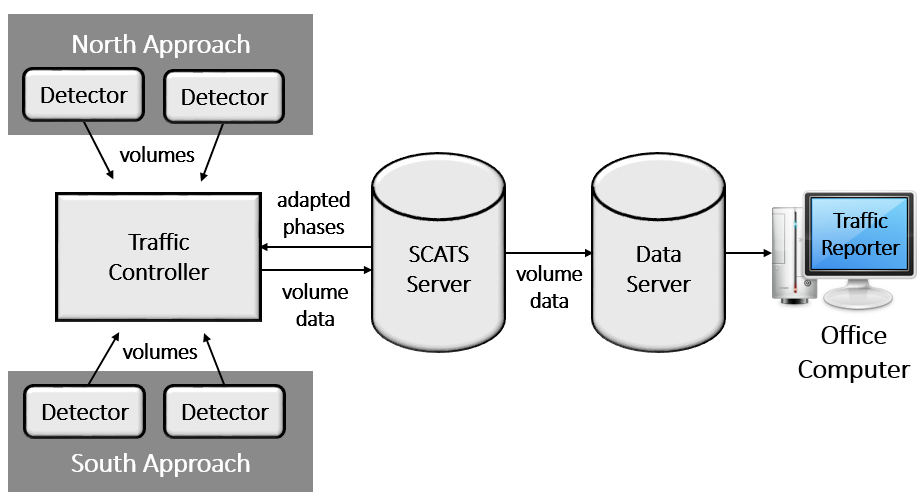
\includegraphics[height=1.8in]{background}}
\caption{Flow diagram of a single intersection}
\label{fig:background}
\end{figure}

The SCATS server can use this volume data to adjust traffic light phases to suit the traffic trends. For example if there is a large volume of traffic headed towards the city centre at a certain intersection, the next intersection will have longer green phases for cars travelling in that direction. While SCATS does lag behind actual traffic trends by 5 minutes, automatically adjusted traffic phases have been shown to be more efficient than statically phased intersections.

As well as adjusting the traffic light phases, the SCATS server also saves the volume data to a data server where it is available for later viewing and analysis in binary *.vs files. Auckland Transport's traffic engineers use an application called Traffic Reporter which can open these files and view the data in a table or graph view.


\section{Requirements}
\subsection{Requirements Gathering}
For this project we have had weekly or fortnightly
meetings with our client. To begin with these meetings were
used to gather requirements and to find out more about how
the existing application works and what it is used for.
The main use of the existing application is to use the
volume data for reports. For example, finding the busiest
intersections for a given month, or finding the busiest time of
day for different intersections, etc.

We also went to the Auckland Transport office in the
Auckland CBD. We saw that it is used in tandem with another
program that directly interfaces with SCATS. The other
program shows detectors being triggered in pseudo real time
and shows planned and actual light phasing. Also available to
them were camera feeds of some of the main intersections.
Using all of these tools they could identify an intersection
whose phasing is incorrect or non-optimal and then check the
volumes of those intersections to see if there are any obviously
faulty detectors.

The visit to Auckland Transport was instrumental in our
understanding of what it is we are trying to replicate and
improve. We were able to identify significantly more use
cases, from seeing the application in action in the environment
that it is used in.

\subsection{Functional Requirements}
From our meetings with our client, we ascertained a number of funtional as well as non-functional requirements. The inital functional requirements were as follows:

\begin{itemize}
	\item Recreate table and graph views
	\item Improve upon these views, giving more details.
	\item Add exporting Microsft Excel
	\item Add the ability to save configurations
\end{itemize}

As the project progressed and time and scope allowed for more features we were given more requirements:

\begin{itemize}
	\item Be able to find suspected faulty detectors
	\item Produce a report over multiple days, giving statistics for each day and averages
\end{itemize}

\subsection{Non-Functional Requirements}

In our intitial meetings there was a big focus on when recreating the application to make it extensible, so that after we had finished the project could be picked up by someone else and continue to work on with little effort.

One of the complaints about the original Traffic Reporter is that it is lacking in aesthetics and usability. One of our client's intentions in having the program recreated was to make it more usable and bring it up to modern standards.

\section{Research}
\subsection{Existing Application}
To recreate the existing application, we had to become
familiar with it. We explored its features and what we liked
and disliked about it.

The current application has two modes; essentially it is two
programs in one. One mode displays information on traffic
volume (the VS mode), the other displays information on the
traffic light phasing. Because of scope constraints we looked
only into the traffic volume part of the application. Later if
time permits, we might look into recreating the phasing part of
the application.

The VS mode has four different views; a graph view, a
table view, a column view, and a dump view. The two most
commonly used views are the graph and table view. We were
unable to ascertain what the column view is actually used for.
The dump view gives a human readable representation of a
volume store file that is very close to how it is encoded. This
was useful to us when we were learning how to read the files,
but is unused otherwise.

The graph view shows a line graph with time on the X-axis
and traffic volume on the Y-axis. Each detector at an
intersection can have it’s own series or they can be grouped
together. The time interval can be set between 5 minutes and
an hour. Data is collected every 5 minutes, so if you increase
the interval it plots the average.

The graph view is useful for seeing trends in traffic flow.
For example for some detectors there is a large spike between
6am and 7am and then it falls off over the rest of the day. We
can look at this and see that that detector probably heads
toward the CBD.

The table view displays volume information for 5-minute
intervals for each hour with hourly totals in the bottom row.
(See Fig.1) There is a table for both AM and PM traffic with
the total for each half of the day and the peak amount and
time. Each approach has its own pair of tables, so like the
graph view you can group detectors together to get an
indication of volume for a specific direction. You can change
the interval to get the totals over that interval.
The table view is good for finding specific values at
specific times, but is poor for identifying trends.
The column view is used only to export data to an Excel
spreadsheet for further manipulation.

\subsection{Potential Solutions}
One of the requirements that the client stressed to us was
future extensibility of platforms. To make the application
portable we initially suggested making a web based
application with a RESTful API [1]. This way it would be
very easy to introduce new platforms that would only have to
make use of the API.

The other choice was a windows desktop application that
loads volume files locally. The main advantage of this
platform choice would be that there would be significantly less
architectural work involved and could be developed more
rapidly. (See Table 1 for pros and cons).

We felt it would be most appropriate to create the
application as a web service. One of the key criteria expressed
by Auckland Transport being extensibility, we felt that a web
service meets this criteria better. Auckland Transport sees this
project as something that is likely to be extended and
improved over the years. Using a web service promotes client
platform in-dependence, which allows Auckland Transport to
reuse the same program for other platforms such as mobile
applications.

Ultimately the client decided to go with a standalone
windows application. This was due to a few factors, the main
ones being that a web service would take longer to create and
that AT was reluctant to grant us access to the infrastructure
required to host such a service.

\section{Traffic Reporter 2013}
\subsection{Improved Features}
\subsubsection{Configuration Screen}
\subsubsection{Table View}
\subsubsection{Graph View}
\subsection{New Features}
\subsubsection{Suspected Faults}
\subsubsection{Summaries}
\subsubsection{CSV Exporting}

\section{Architecture}
\subsection{Presentation Logic}
\subsection{Data Sources}
\section{Reflections}
\section{Conclusions}

\section{Future Work}

\bibliographystyle{IEEEtran}
\bibliography{final_report}


\end{document}